\documentclass{article}
\usepackage[utf8]{inputenc} % allow utf-8 input

%\usepackage{arxiv}

% basic stuff it's always nice to have
\usepackage{xcolor}
\usepackage{amsmath}
\usepackage[T1]{fontenc}    % use 8-bit T1 fonts
\usepackage{hyperref}       % hyperlinks
\usepackage{url}            % simple URL typesetting
\usepackage{booktabs}       % professional-quality tables
\usepackage{amsfonts}       % blackboard math symbols
\usepackage{nicefrac}       % compact symbols for 1/2, etc.
\usepackage{microtype}      % microtypography
\usepackage{graphicx}
\usepackage{lmodern}

\usepackage{cleveref}       % use for references

% nice bibliography stuff
\usepackage{natbib}
\usepackage{doi}

\usepackage{lineno}         % add line numbers
\usepackage{authblk}        % nicely format authors

% This is for code listings. Edit the file listings-options.sty to change the default settings.
\usepackage{listings}
\usepackage{listings-options}

% Lets you write \argmax in equations
\DeclareMathOperator{\argmax}{argmax} 

% Formatting links
\hypersetup{colorlinks = true,
linkcolor = purple,
urlcolor  = blue,
citecolor = cyan,
anchorcolor = black}

% use \todo to put notes in the margin to co-authors, or \longtodo to put in main body
\newcommand{\todo}[1]{\marginpar{\scriptsize\color{red}\raggedright #1}}
\newcommand{\longtodo}[1]{{\color{red} #1}}

% use these to format differential equations to make Dan happy because the d should not be italic
\newcommand{\ud}{\mathrm{d}}
\newcommand{\dt}{\ud t}

% Purely stylistic stuff, please feel free to change as you like
\renewcommand\Affilfont{\itshape\small}
\addtolength{\marginparwidth}{0.5cm} \addtolength{\hoffset}{-2cm}
\addtolength{\textwidth}{3cm} \addtolength{\voffset}{-2cm}
\addtolength{\textheight}{4cm} \setlength{\parindent}{0pt}
\setlength{\parskip}{1.3ex}

%%%%%%%% Figure placement controls (see https://aty.sdsu.edu/bibliog/latex/floats.html)
% Alter some LaTeX defaults for better treatment of figures:
% See p.105 of "TeX Unbound" for suggested values.
% See pp. 199-200 of Lamport's "LaTeX" book for details.
%   General parameters, for ALL pages:
\renewcommand{\topfraction}{0.9}	% max fraction of floats at top
\renewcommand{\bottomfraction}{0.8}	% max fraction of floats at bottom
%   Parameters for TEXT pages (not float pages):
\setcounter{topnumber}{2}
\setcounter{bottomnumber}{2}
\setcounter{totalnumber}{4}     % 2 may work better
\setcounter{dbltopnumber}{2}    % for 2-column pages
\renewcommand{\dbltopfraction}{0.9}	% fit big float above 2-col. text
\renewcommand{\textfraction}{0.07}	% allow minimal text w. figs
%   Parameters for FLOAT pages (not text pages):
\renewcommand{\floatpagefraction}{0.7}	% require fuller float pages
% N.B.: floatpagefraction MUST be less than topfraction !!
\renewcommand{\dblfloatpagefraction}{0.7}	% require fuller float pages
% remember to use [htp] or [htpb] for placement

%%%%%%%%%%%%%%%%%%%%%%%%%%%%%%%%%%%%%%%%%%%%%%%%%%%%%%%%%%%%%%%%%%%%
%%%%%        TITLE AND AUTHORS                               %%%%%%%
%%%%%%%%%%%%%%%%%%%%%%%%%%%%%%%%%%%%%%%%%%%%%%%%%%%%%%%%%%%%%%%%%%%%
\title{New project article template}
\author[1]{A. N. Other}
\author[1]{Dan F. M. Goodman}
\affil[1]{Imperial College London}

% Uncomment to remove the date
\date{}

% Turn on line numbers
%\linenumbers

\begin{document}
\maketitle

%%%%%%%%%%%%%%%%%%%%%%%%%%%%%%%%%%%%%%%%%%%%%%%%%%%%%%%%%%%%%%%%%%%%
%%%%%        START OF DOCUMENT                               %%%%%%%
%%%%%%%%%%%%%%%%%%%%%%%%%%%%%%%%%%%%%%%%%%%%%%%%%%%%%%%%%%%%%%%%%%%%

\begin{abstract}
	\begin{itemize}
        We set up a new project in LaTeX with some good standard ways of doing stuff.
	\end{itemize}
\end{abstract}

\section{Introduction}\label{sec:introduction}

\todo{Are citations really great?}
Citations are great \citep{Goodman2009,perez-nieves_sparse_2021}.
\citet{Goodman2009} say that citations are great anyway (at least they are if you use the right macro; \citealt{perez-nieves_sparse_2021}). Use \texttt{\textbackslash{}citep} to cite in parentheses, \texttt{\textbackslash{}citet} to cite in text, and \texttt{\textbackslash{}citealt} to cite without parentheses (e.g. if your citation is already in parentheses).

\begin{equation}
    \argmax_{x} f(x)
    \label{eq:argmax}
\end{equation}

\Cref{eq:argmax} is a great equation (and so is \cref{eq:argmax}). If you use the \texttt{\textbackslash{}Cref} and \texttt{\textbackslash{}cref} commands from the \texttt{cleveref} package, you can automatically get the right kind of reference and it's easy to update if journal requirements are different without rewriting every reference by hand. Works for things like sections and figures too, e.g. \cref{sec:results}, \cref{fig:elephant}.

Note on labels: use labels like \texttt{sec:introduction} to make it easy to see at a glance what you're referencing where. NEVER use a number in a label because your label \texttt{fig1} will probably not be figure 1 in the final version. Don't do this for figure filenames either!

\longtodo{This is a long todo that will be in the main body of the text.}

\begin{figure}[!htbp]
    \centering
    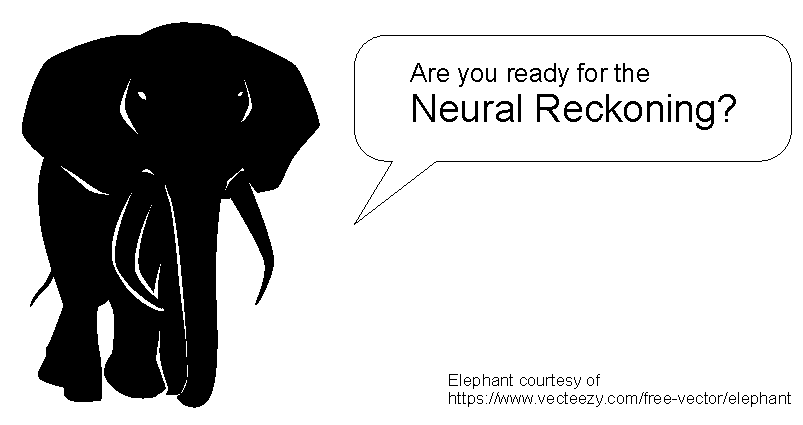
\includegraphics[width=0.5\linewidth]{figures/elephant.pdf}
    \caption{Elephants never forget.}
    \label{fig:elephant}
\end{figure}

\section{Results}\label{sec:results}

\subsection{Every subsection should be a result}

\subsection{The titles of the subsections should tell a short story}

\subsection{And you should probably have one figure per subsection}

\section{Methods}\label{sec:methods}

When writing your text, don't assume that the methods will be before or after the results because this might be different for different journals.

\section{Discussion}\label{sec:discussion}

\section*{Acknowledgements}\label{sec:acknowledgements}

\bibliographystyle{unsrtnat}
\bibliography{paper.bib}

\end{document}